\documentclass{article}

\usepackage[%
    left=0.5in,%
    right=0.5in,%
    top=0.5in,%
    bottom=0.5in,%
]{geometry}%
\usepackage{minitoc}
\usepackage{multicol}
\usepackage{graphicx}
\usepackage{fixltx2e}
\usepackage{listings}
\usepackage{color}
\usepackage{hyperref}
    \hypersetup{ colorlinks = true, linkcolor = blue }
\usepackage{blindtext}
\definecolor{lightgray}{gray}{0.9}
\graphicspath{ {./} }

\newcommand{\inlinecode}[2]{\colorbox{lightgray}{\lstinline
[language=#1]$#2$}}
\newcommand{\worddef}[1]{\hyperref[sec:reference]{\textit{#1}}}

\begin{document}

\tableofcontents

\newpage

\section{Block Ciphers}
\begin{itemize}
  \item Block ciphers use a key to encrypt a fixed-size block of plaintext into a fixed-size block of ciphertext 
  \item If you’re careful, you can convert between block and stream ciphers using modes of operation
\end{itemize}

\section{SP-Networks}
\begin{itemize}
  \item Claude Shannon suggested that all that was required for a strong cipher was repeated \textbf{substitution and permutation} 
  \item SP-Networks combine a substitution process with a permutation into a single round 
  \item Rounds are then repeated enough times to ensure the algorithm is secure
  \item \textbf{Substitution Boxes} – Add confusion by replacing values with other values using a lookup table
  \begin{center}
    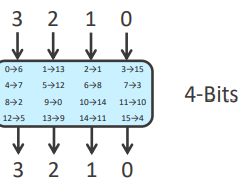
\includegraphics[scale=0.5]{subst_box.png}
  \end{center}
  \item \textbf{Permutation Boxes} – Add diffusion by moving values around from input to output
  \begin{center}
    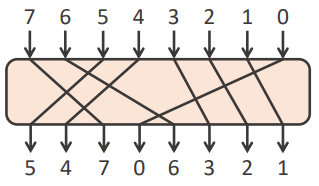
\includegraphics[scale=0.5]{perm_box.png}
  \end{center}
  \item Combined, result in:
  \begin{center}
    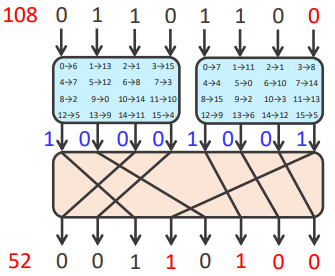
\includegraphics[scale=0.5]{sp_box.png}
  \end{center}
\end{itemize}

\subsection{Notes}
\begin{itemize}
  \item One Round \textbf{isn’t enough}! 
  \item Careful analysis of input changes and output changes can reveal the contents of the S-boxes 
  \item More rounds produces more diffusion 
  \item Replacing permutation with linear transformation is more effective. Each bit is the XOR combination of multiple S-box outputs
  \item Typically the box size is around 128-bit and 256-bit.
  \item "Psuedorandomness" of the result is compromised with poor S-box design
\end{itemize}

\subsection{Key Mixing}
\begin{flushleft}
The previous SP-network didn’t use a key, we can add one using XOR:
\end{flushleft}
\begin{center}
  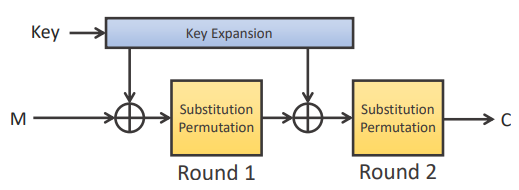
\includegraphics[scale=0.5]{key_mix.png}
\end{center}


\section{Advanced Encryption Standard}
\begin{itemize}
  \item Superseded DES as a standard in 2002. A standard built around the Rijndael algorithm 
  \item Rijndael is an SP-Network with a 128-bit block size, and a key length of 128, 192 or 256-bits 
  \item Round count depends on key length. 10, 12 or 14 cycles
  \item AES is vastly superior to DES, which had a 64-bit block and 56 bit key
  \item AES uses rounds of 4 layers, and a final round of 3. Bytes are represented as a 4x4 block called the state
\end{itemize}

\begin{center}
  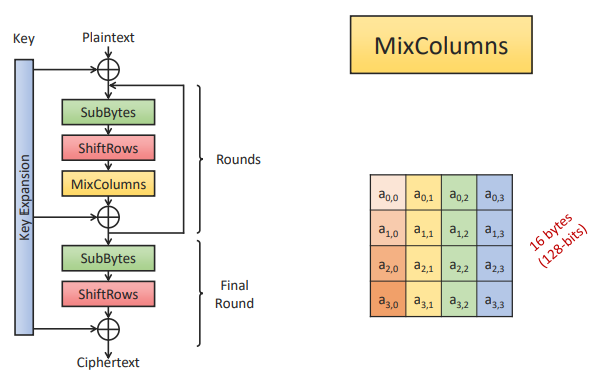
\includegraphics[scale=0.5]{aes.png}
\end{center}

\section{Block Cipher Modes}
\begin{itemize}
  \item Most messages don’t come in convenient 128-block lengths 
  \item We’ll need to run a block cipher repeatedly on consecutive blocks
\end{itemize}

\subsection{Electronic Code Book (ECB)}
\begin{itemize}
  \item Just encrypt each block one after another 
  \item Weak to redundant data divulging patterns
\end{itemize}
\begin{center}
  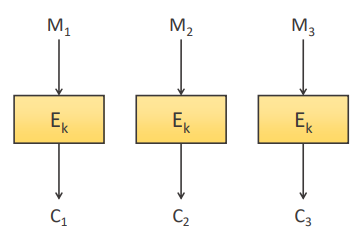
\includegraphics[scale=0.5]{ecb.png}
\end{center}

\subsection{Cipher Block Chaining (CBC)}
\begin{itemize}
  \item XOR the output of each cipher block with the next input 
  \item Not totally immune to the insertion of malicious blocks
\end{itemize}
\begin{center}
  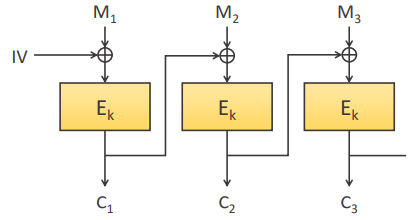
\includegraphics[scale=0.5]{cbc.png}
\end{center}

\subsection{Counter Mode (CTR)}
\begin{itemize}
  \item Encrypting a counter 
  \item Can be parallelized! 22 to produce a stream cipher
\end{itemize}
\begin{center}
  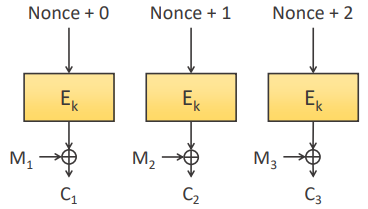
\includegraphics[scale=0.5]{ctr.png}
\end{center}

\subsection{Galois Counter Mode (GCM)}
\begin{itemize}
  \item Extends counter mode to add authenticity: the sender definitely sent that message, and it hasn’t changed 
  \item Very similar to counter mode, but adds an authentication tag 
  \item The tag is calculated using multiplication in a Galois Finite field GF(2128) 
  \item Extremely parallelisable and robust to message alteration
\end{itemize}

\section{Cryptographic attack models}
\begin{flushleft}
Attack models weakest to strongest
\end{flushleft}
\begin{itemize}
  \item Brute-force 
  \item Ciphertext-only 
  \item Known-plaintext 
  \item Chosen-plaintext 
  \item Chosen-ciphertext 
  \item Related-key attack
\end{itemize}

\pagebreak
\section*{Reference section} \label{sec:reference}
\begin{description}
	\item[placeholder] \hfill \\
\end{description}
\end{document}
